\begin{figure}[h!]
    \centering
    \caption{Average rent, square footage, and rent per square foot by household 
             income decile, renters sample}
    \label{fig:ahs_rent_sqft}

    \begin{subfigure}{.69\textwidth}
        \caption{Average residualized rent per square footage}
        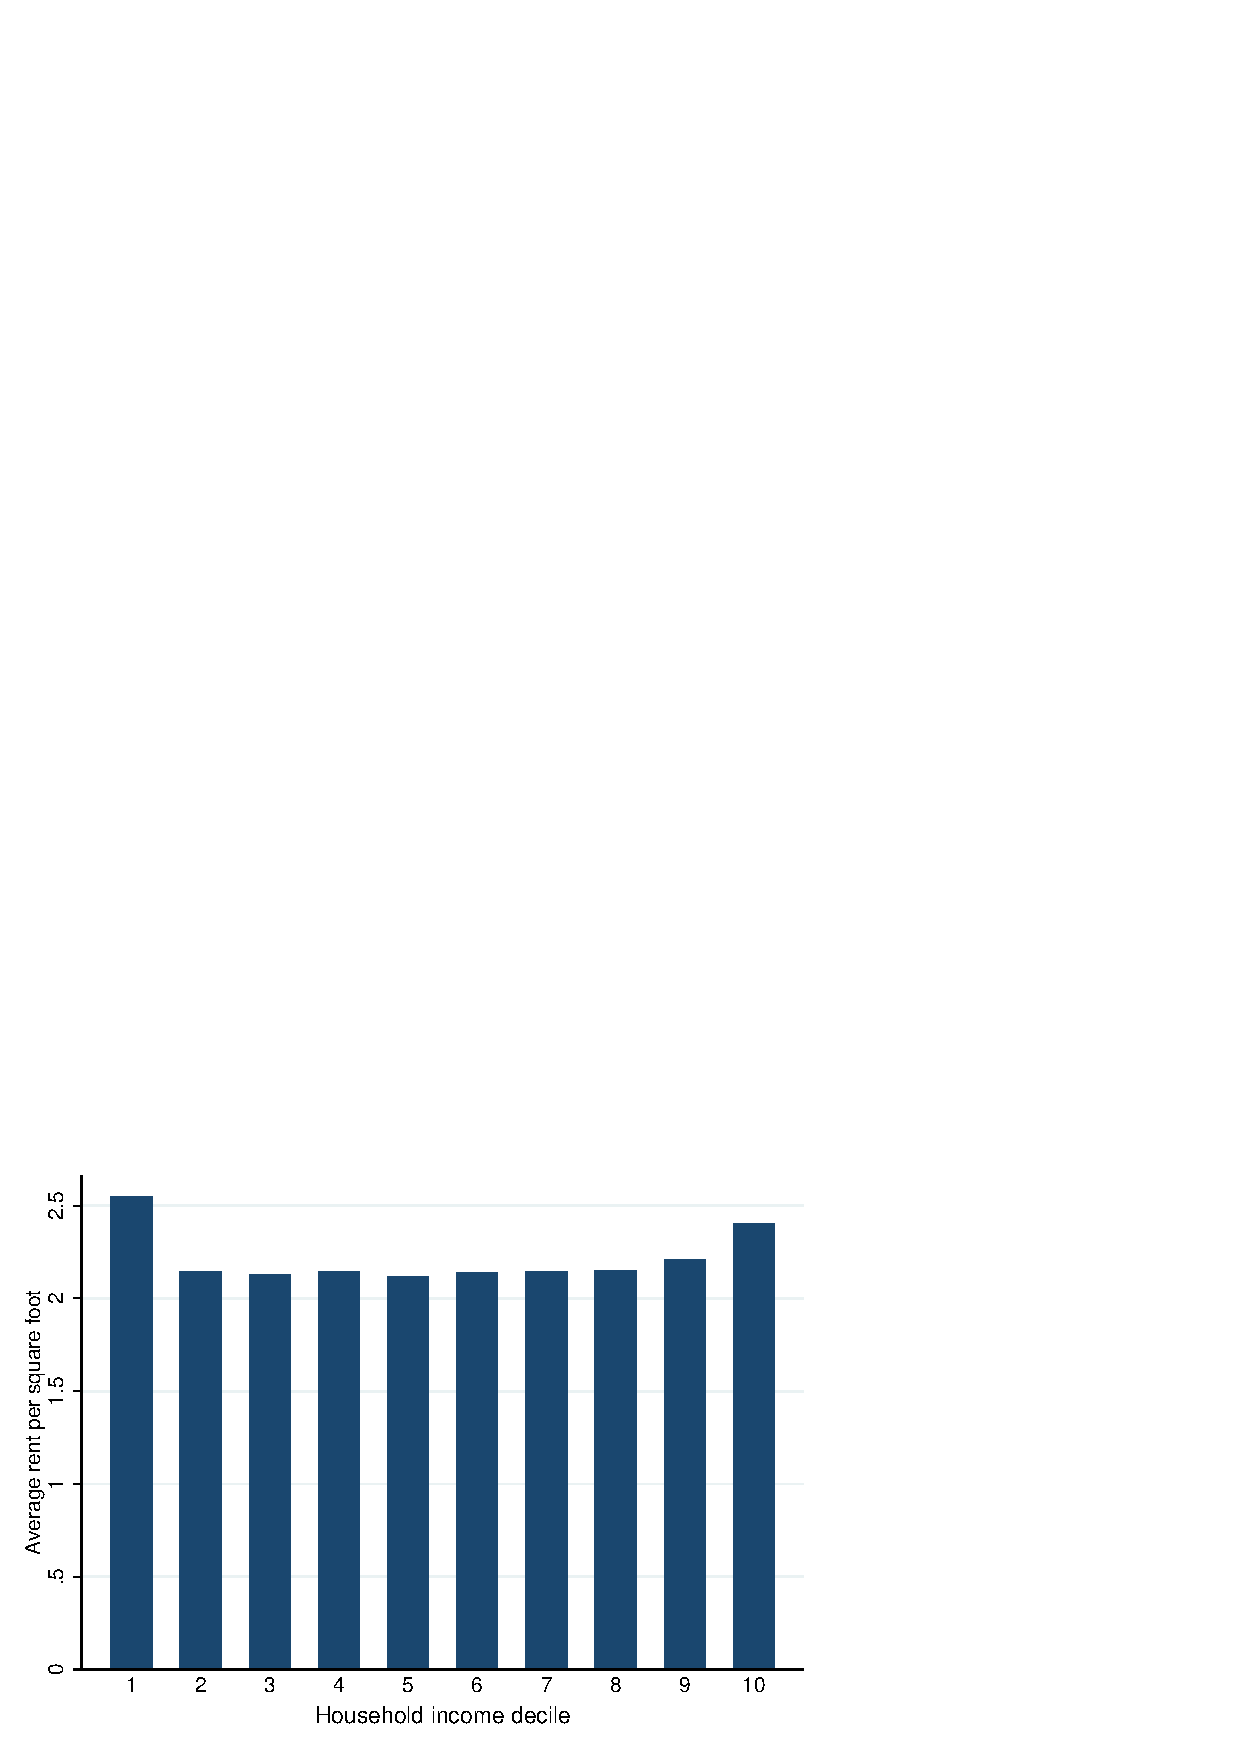
\includegraphics[width = 1\textwidth]
            {ahs/output/avg_rent_psqft}
    \end{subfigure}\\
    \begin{subfigure}{.48\textwidth}
        \caption{Average residualized rent}
        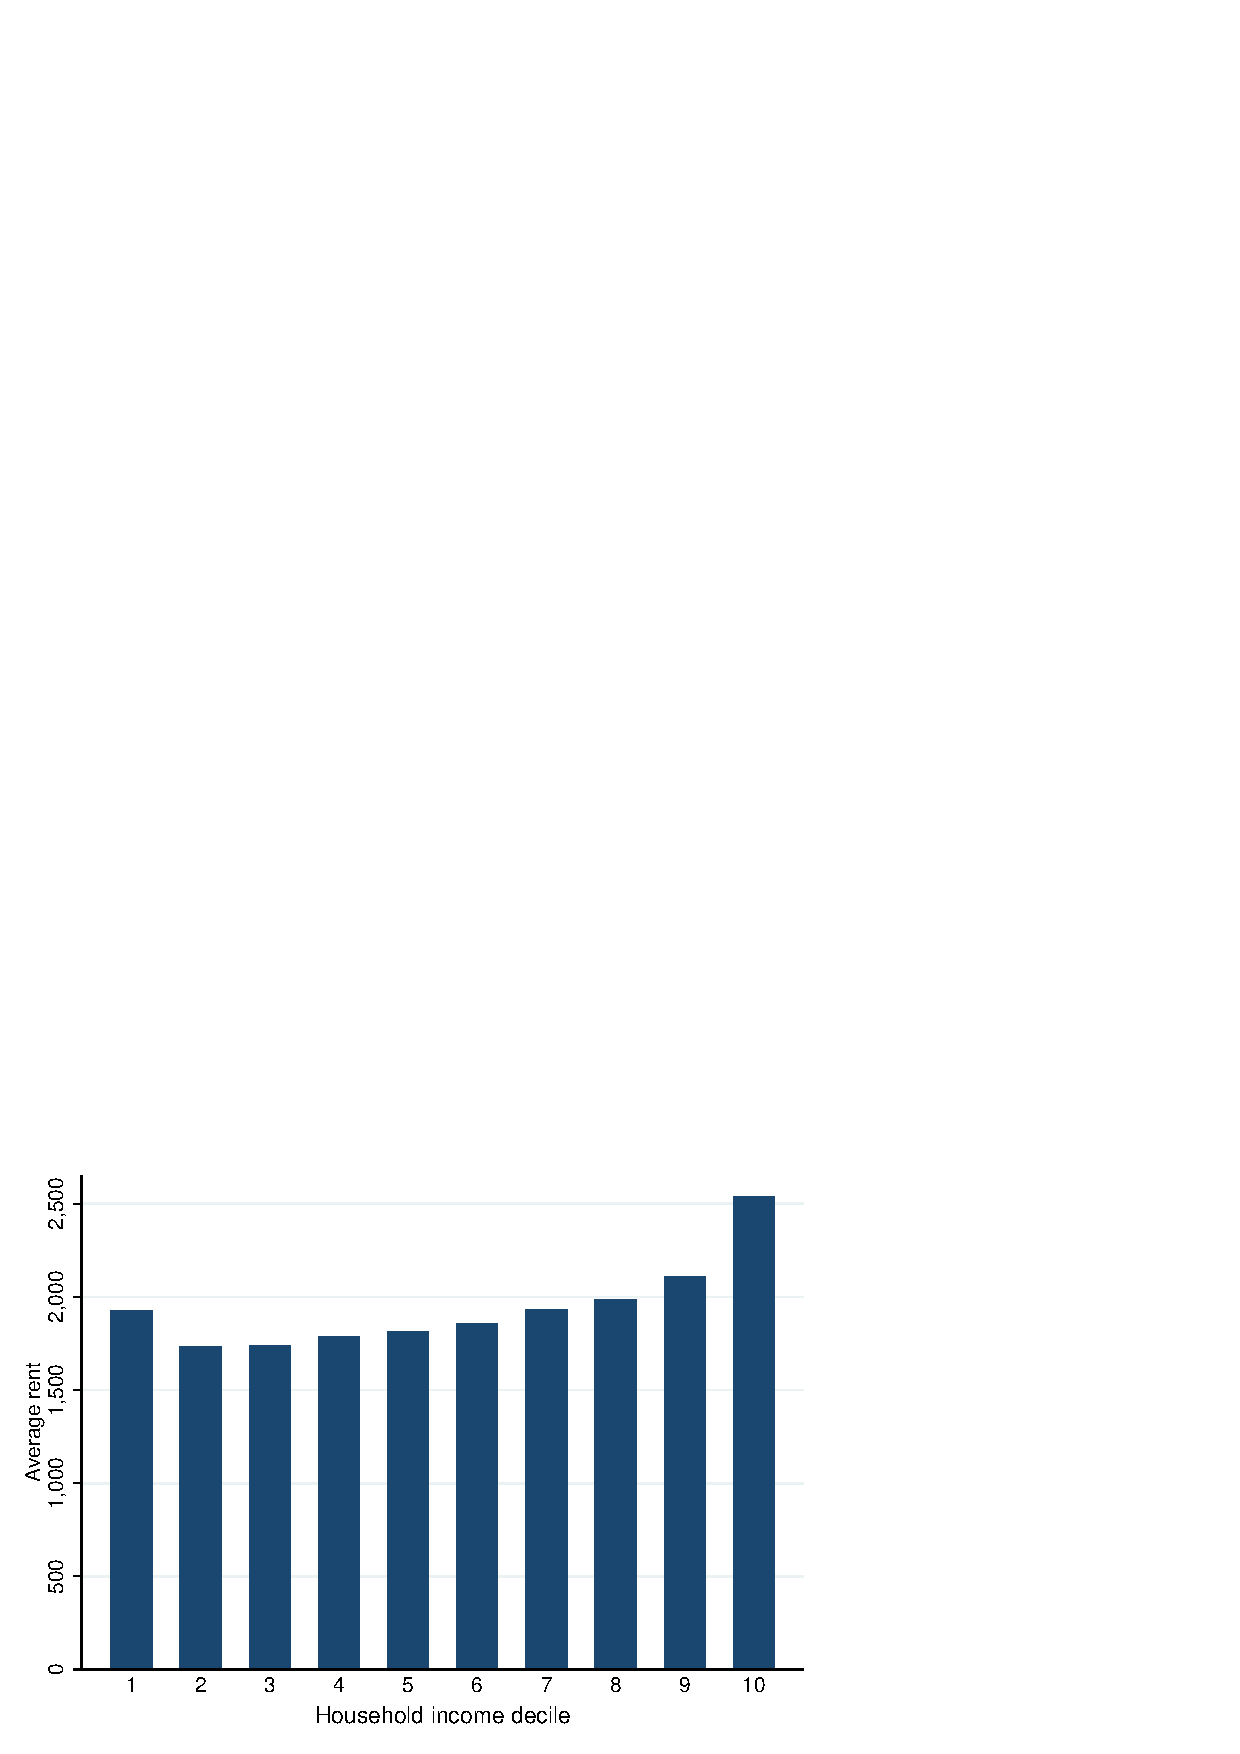
\includegraphics[width = 1\textwidth]
            {ahs/output/avg_rent}
    \end{subfigure}%
    \begin{subfigure}{.48\textwidth}
        \caption{Average residualized square foot}
        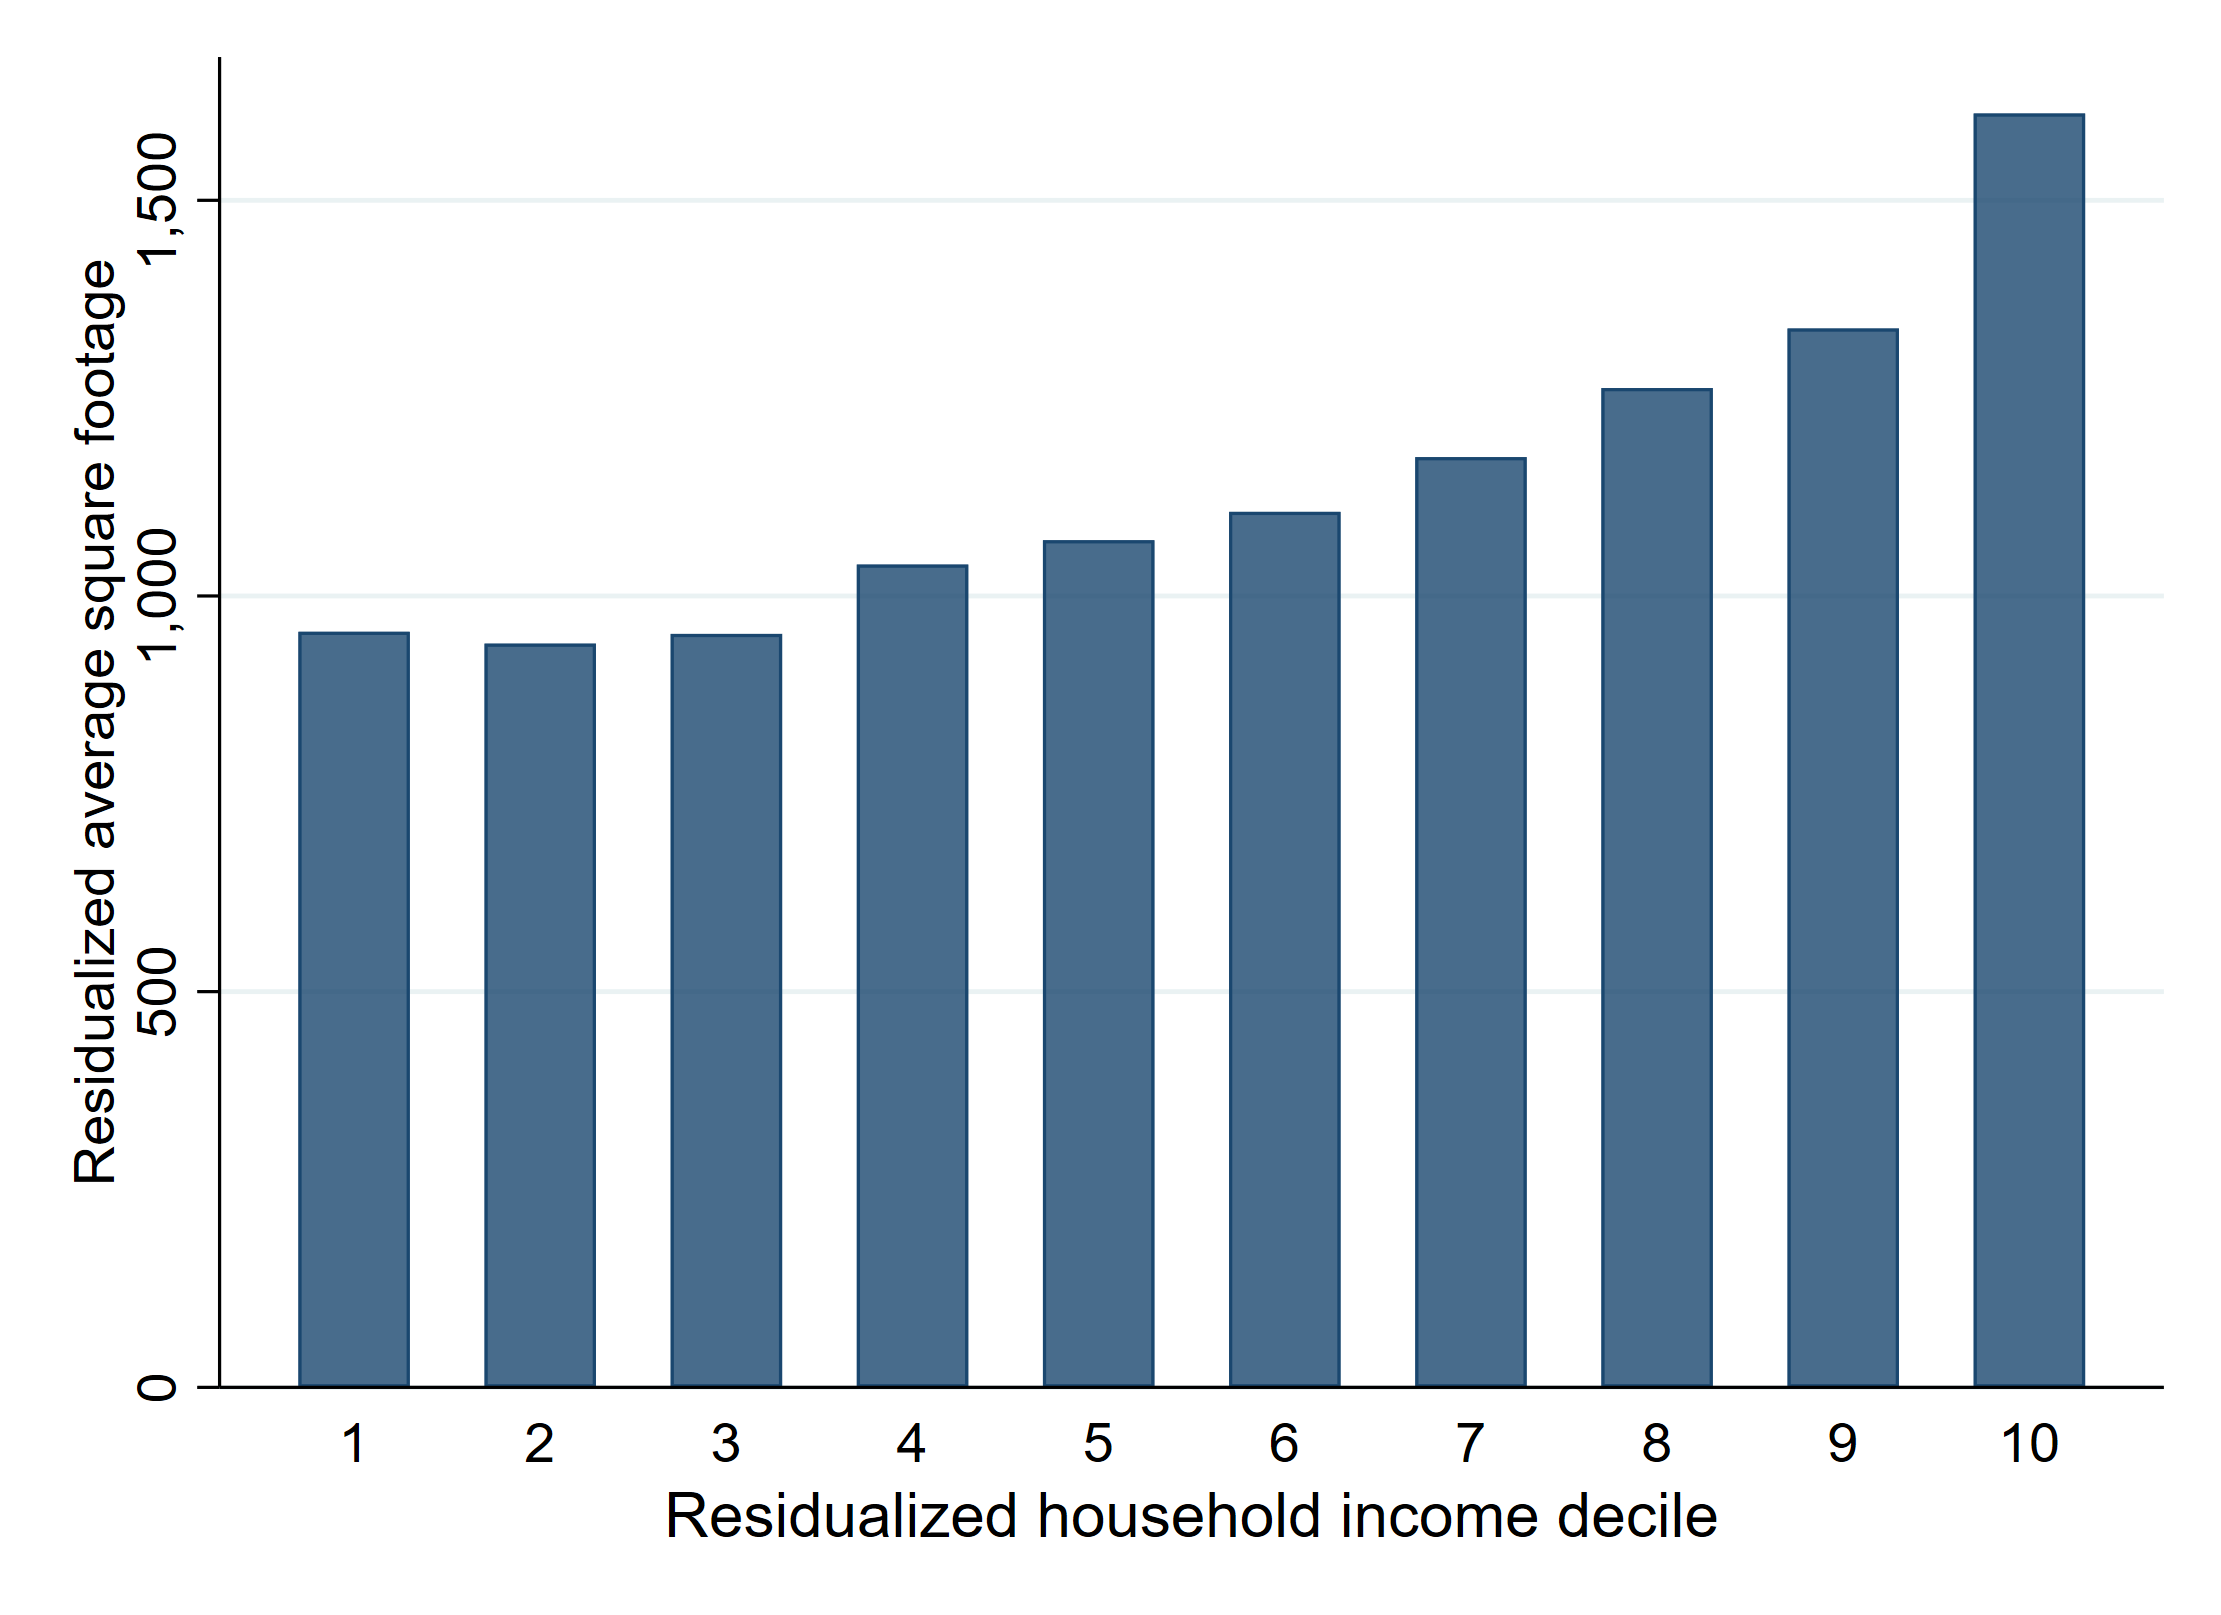
\includegraphics[width = 1\textwidth]
            {ahs/output/avg_sqft}
    \end{subfigure}

    \begin{minipage}{.95\textwidth} \footnotesize
        \vspace{3mm}
        Notes: Data are from the 2011 and 2013 American Housing
        Survey \parencite{ahs2020}. 
        The top left figure shows the average rent by household 
        income, the top right figure shows the average square 
        footage by household income, and the bottom figure shows
        the average rent per square footage by household income.
        We construct the figure as follows. 
        First, we residualize the variable in the y-axis and household 
        income by SMSA, a concept of metropolitan areas available in the 
        data.
        Second, we construct deciles of the residualized household
        income variable.
        Finally, we take the average of the residualized y-variable
        within each decile.
        The sample of individuals includes rented households with 
        non-missing values in square footage and rental payments.
        We exclude from the calculation non-conventional housing units, 
        such as mobile homes, hotels, and others.
    \end{minipage}
\end{figure}
